\documentclass[a4paper,12pt]{article}
\usepackage{graphicx} 
\usepackage{amsmath} 
\usepackage{amssymb} 
\usepackage{geometry} 
\usepackage{fancyhdr} % for headers and footers
\usepackage{caption} % for customizing captions
\usepackage{setspace} 
\usepackage{enumitem} % for customizing lists
\usepackage{biblatex} % for bibliography
\usepackage[colorlinks,linkcolor=blue,citecolor=blue,urlcolor=blue]{hyperref}
\addbibresource{references.bib} % specify your bibliography file


\geometry{margin=1in}
\setlength{\parindent}{0pt}
\setlength{\parskip}{6pt}
\doublespacing

 
\pagestyle{fancy}
\fancyhf{}
\fancyhead[L]{\leftmark}
\fancyfoot[C]{\thepage}

 
\newcommand{\customtitlepage}{
    

    \begin{titlepage}
        
\includegraphics[width=0.9\textwidth]{logo.png}\\
        \centering
        \vspace*{1cm}
        
        \Huge\textbf{A Basic Study of Dimensionality}\\
        \vspace{0.5cm}
        \LARGE\textit{A Quantitative Approach}\\
        \vspace{1.5cm}
        
        \textbf{Scientific Data Acquisition and Processing} \\
        \textbf{Instructor Name:} Riccardo Barberi\\
        \vspace{0.5cm}
        
        \textbf{Authors:}\\
        \large Michele Arcuri, Luca Coscarelli, Nelson Manuel Mora Fernández\\
        \vfill
        
        \large \textbf{Date of Submission:}\\
        \today\\
        \vspace{1.5cm}
        
        \small
        Department of Physics \\
        University of Calabria\\
        \vspace{0.5cm}
    \end{titlepage}
}

\begin{document}

% Title page
\customtitlepage

% Abstract
\begin{abstract}
    A brief summary of the experiment.
\end{abstract}


% Keywords
\section*{Keywords}
List of relevant keywords 

\newpage

% Table of Contents
\tableofcontents
\newpage

% Introduction
\section{Introduction}
In the following experiment our aim is to demonstrate the fractal nature 
of a very simple physical object: a small tin foil ball. 

Fractal objects are objects which are characterised of the self-similarity 
property, in simpler words, they look the same when observed at different scales.
One of the most famous fractal object is the Mandelbrot set, but we can find these 
objects also in nature, such as in the structure of a Romanesco Caullflower, or 
from a physical point of view, polymers can be regarded as fractals as well.

\begin{figure}
    \centering
    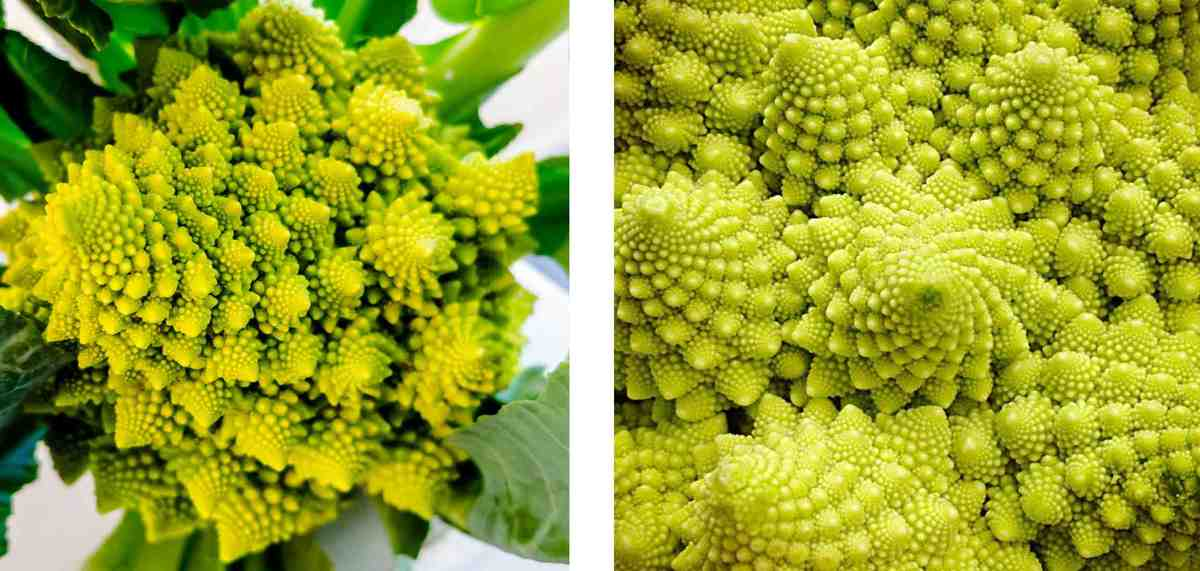
\includegraphics[width = 0.8\textwidth]{..\foto\Cauliflower.jpg}
    \caption{An example of cauliflower seen from far away (left) and from up close (right)}
    \label{fig:Cauliflower}
\end{figure}

\begin{figure}
    \centering
    \begin{minipage}{1\textwidth}
        \centering
        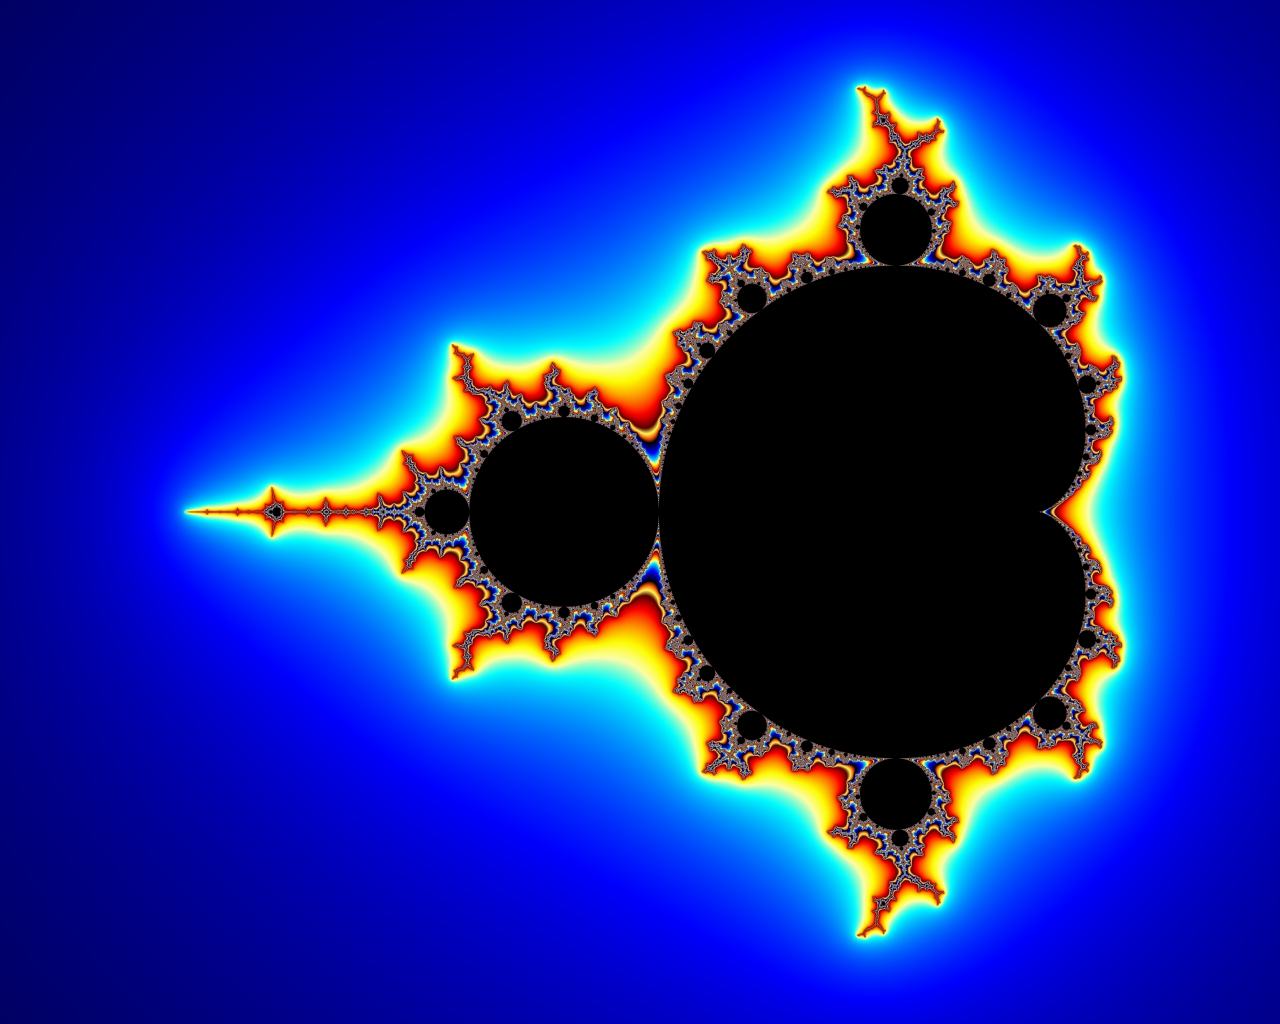
\includegraphics[width = 0.45\textwidth]{..\foto\Mandelbrot_far.jpg}
        \includegraphics[width = 0.45\textwidth]{..\foto\MAndelbrot_close.jpg}
    \end{minipage}
    \caption{The Mandelbrot set seen from far away (left) and from up close (right)}
    \label{fig:Mandelbrot}
\end{figure}

We can observe the same level of complexity of the images as seen from far away 
and up close in Fig \ref{fig:Cauliflower} and Fig \ref{fig:Mandelbrot} above.

From the mathematical point of view, we have to define a fractal from its changes 
in terms of mass and volume. We start from an object that we know: a square sheet 
of paper. In this case we will have the mass distributed following the area of 
the sheet, furthermore the mass grows as the square of the typical lenght of the 
sheet (the side of the square which we will call $r$). The formula will be the 
following 
\[ M = C r^2 \]
where $C$ is the surface density of the material of the sheet.

We can repat the same reasoning with a metal cube, obtaining ultimately the formula
\[ M = D r^3 \]
where $D$ is the volume density of the metal used. 

Now let's apply this method to our experiment. Since the physical data which we 
will obtain will be the mass and the linear dimension of the system 
(the tin foil ball) the parameters will be the general density $k$ and 
the exponent $\alpha$ in the formula
\begin{equation} 
    M_{\text{exp}} = k r_{\text{exp}}^{\alpha}
    \label{eq:gen_fractal}
\end{equation}   

To sum up, in the following experiment we will see that also a rolled up ball of 
tin foil can be considered as a fractal.


% Materials and Methods (Tools and Procedure)
\section{Materials and Methods}
\subsection{Equipment and Tools}
\begin{itemize}
    \item Precision balance
    \item Caliber
    \item Micrometer
    \item Drawing rule and / or square
    \item Scissors
    \item Aluminum foil
\end{itemize}
\subsection{Experimental Procedure}
Detail the step-by-step process followed during the experiment, including any setup instructions, procedures, and configurations.

% Results (Graphs and Data)
\section{Results}
Present all data collected, including graphs, tables, or charts. Explain the trends and observations found during the experiment.

% Discussion and Analysis
\section{Discussion and Analysis}
Interpret the results, compare them with expected outcomes, and discuss any deviations or unexpected findings. Address possible sources of error and suggest improvements.

% Conclusion
\section{Conclusion}
Summarize the main findings, confirm or refute the hypothesis, and suggest future research directions or practical applications.

% Appendix
\section{Appendix}
Include supplementary information such as raw data, calculations, or additional graphs that are too detailed for the main report but are still relevant.

% References
\printbibliography

\end{document}
